\documentclass{article}
\usepackage{hyperref}
\usepackage{dsfont}
\usepackage{graphicx}
\usepackage{color, soul}
\usepackage{amsmath}
\title{Can COViD steal Bob's idea?}
\author{My Little Trojan}

\begin{document}
	\maketitle
	\noindent
	Cryptography challenge from \textbf{STACK the Flags 2020}.\\
	
	\section{The Challenge}
	Bob wants Alice to help him design the stream cipher's keystream generator base on his rough idea. Can COViD steal Bob's "protected" idea?\\
	\\
	\textbf{File provided:} 1x PCAPNG file that stores a dump of packets captured over a network\\
	\\
	\textbf{Expected Flag}: Numeric String
	
	\section{Tools Used}
	\begin{enumerate}
		\item 
		\href{https://www.wireshark.org/download.html}{Wireshark}: Good and free pcapng viewer.
		\item
		Discrete Logarithm Calculator: \url{https://www.alpertron.com.ar/DILOG.HTM}
		\item
		Python Console: For doing math on large numbers
	\end{enumerate}
	
	\section{The Hack}
	\subsection{The Wireshark Interface}
	After launching Wireshark, you will get a list view of all the packets. After scrolling about, you should notice a message in packet 52.
	
	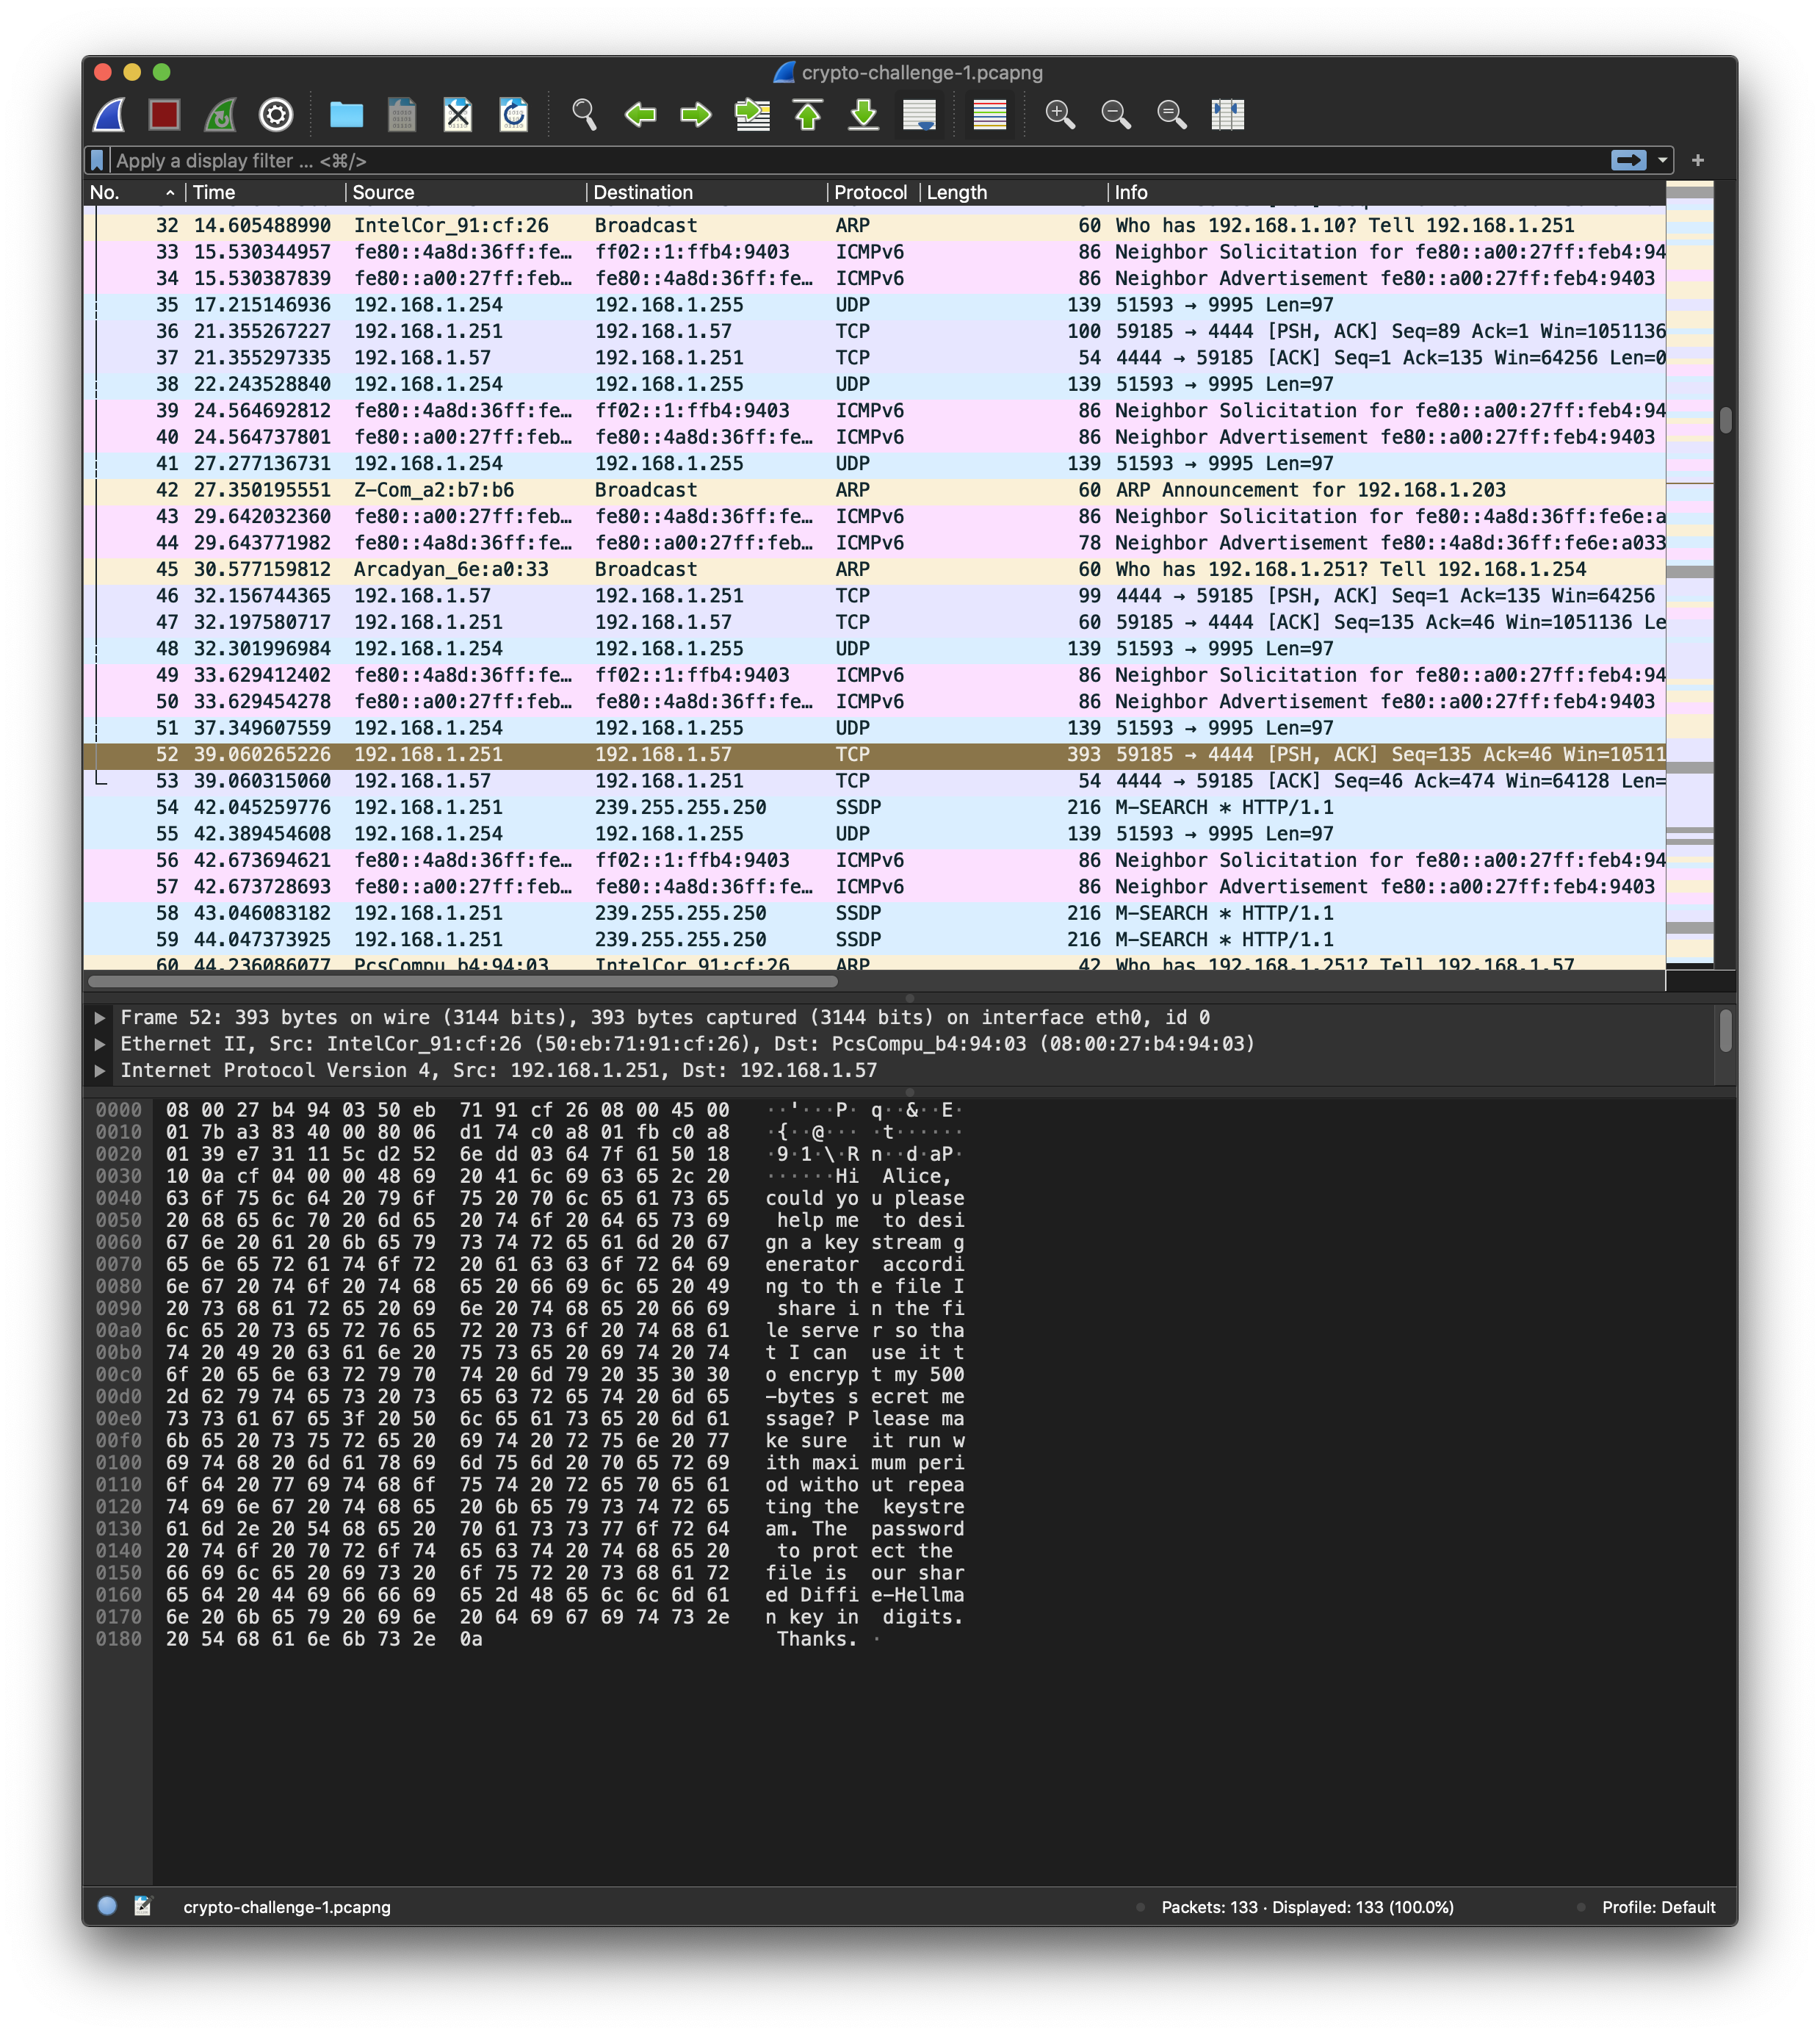
\includegraphics[width=\textwidth,height=\textheight,keepaspectratio]{wireshark}
	The message in the rightmost column reads:\\
	\texttt{Hi Alice, could you please help me to design a keystream generator according to the file I share in the file server so that I can use it to encrypt my 500-bytes secret message? Please make sure it run with maximum period without repeating the keystream. \hl{The password to protect the file is our shared Diffie-Hellman key in digits.} Thanks.}
	
	\subsection{Diffie-Hellman key exchange}
	This is a cryptographic method that involves large prime numbers and modular arithmetic that was published in 1976.
	\begin{enumerate}
		\item Alice and Bob publicly agree to use a modulus $p$ and generator $g$ (that generates the cyclic group $\mathds{Z}/p\mathds{Z}$)
		\item Alice chooses a secret integer $a$ and sends Bob $A = g^a\ mod\ p$
		\item Bob chooses a secret integer $b$ and sends Alice $B = g^b\ mod\ p$
		\item Alice and Bob would be able to arrive at a shared secret $s$ like so:
		\[
			s=A^b\ mod\ p=B^a\ mod\ p=g^{ab}\ mod\ p
		\]
	\end{enumerate}
	We are to look out for the publicly available $p, g, g^a, g^b$. Once we have these information, we can use the Discrete Logarithm Calculator to work out $a$ or $b$ to calculate \hl{$g^{ab}\ mod\ p$}.
	
	\subsection{Computation}
	After scouring the packets, you should have found the 4 public numbers:
	\begin{itemize}
		\item $p$ = 298161833288328455288826827978944092433
		\item $g$ = 216590906870332474191827756801961881648
		\item $g^a$ = 181553548982634226931709548695881171814
		\item $g^b$ = 64889049934231151703132324484506000958
	\end{itemize}
	We now compute $a$.\\
	
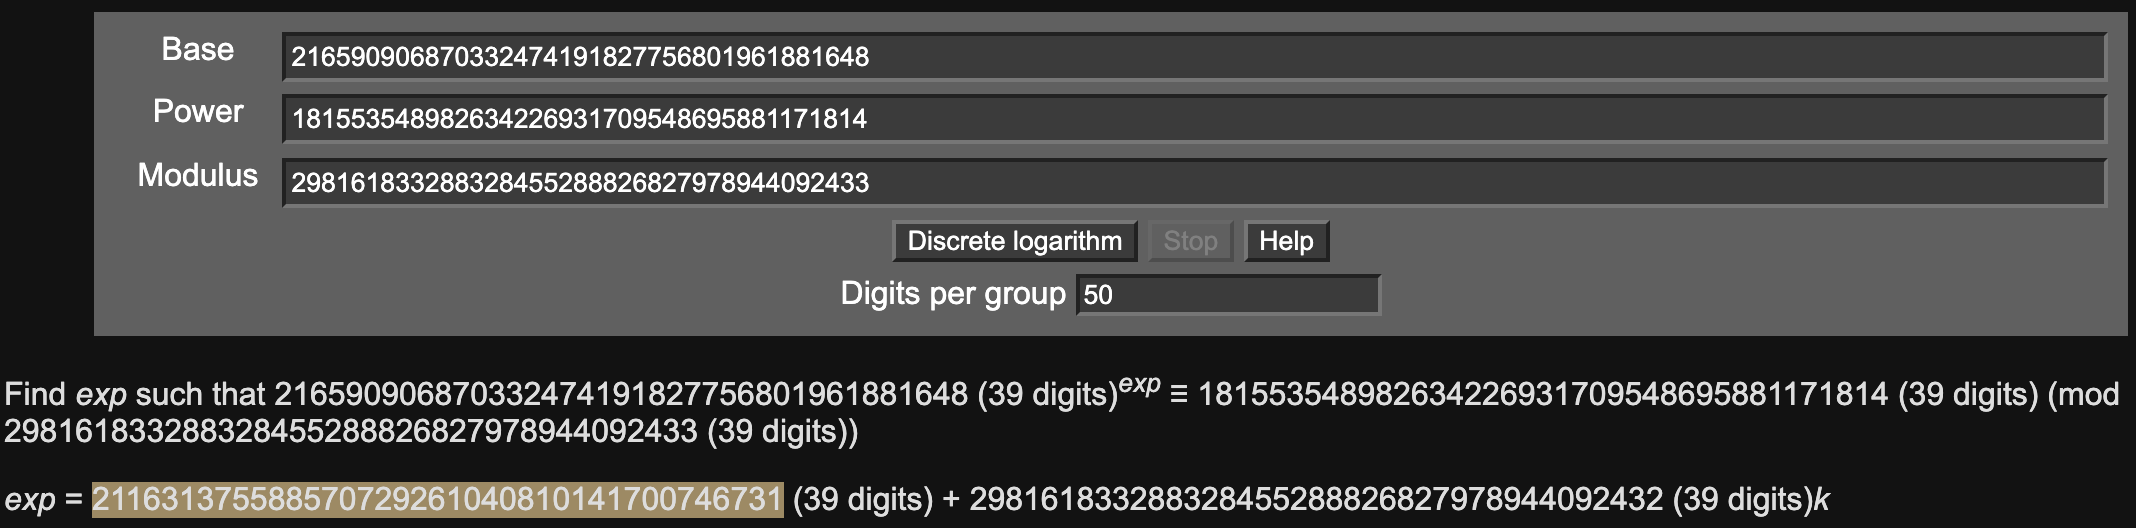
\includegraphics[width=\textwidth,height=\textheight,keepaspectratio]{dilog}\\
\[
a=211631375588570729261040810141700746731
\]
Lastly, using Python Console we easily compute $(g^b)^a\ mod\ p$ using the pow function, i.e. \texttt{pow($g^b$, $a$, $p$)}.\\ We arrive at the flag, \textbf{246544130863363089867058587807471986686}.

\newpage
\textbf{\LARGE{Appendix: Pohlig-Hellman Algorithm}}
\\
\\
This is the algorithm used by the Discrete Logarithm Calculator. Here we provide a worked example with small numbers to show how it is done.
\[
\beta=\alpha^x\ mod\ p,\ 0\leq x\leq p-1
\]
Let $p=41,\ \alpha=7,\ \beta=12$, i.e. \hl{$12=7^x\ mod\ 41$}. Solve for $x$.

\begin{enumerate}
	\item Find the prime factors of Euler totient function, $\varphi(p)$. We know $p$ is prime, so
	\[
	\varphi(p)=p-1=2^3\cdot5
	\]
	\[
	q=\{2,5\}
	\]
	\item Find a congruence for prime factor, $q$.
	\item For $q=2$, $x=2^0\cdot x_0+2^1\cdot x_1+2^2\cdot x_2$, $x$ has 3 terms as 2 has power 3.
	\begin{itemize}
		\item Solving for $x_0$,
		\begin{align}
		\beta^{\frac{p-1}{q}} &= \alpha^{\frac{p-1}{q}x_0} \\
		12^{20} & = 7^{20x_0} \\
		-1\ (mod\ 41) &= (-1)^{x_0}\ (mod\ 41) \\
		\text{Test } x_0=0,1,2,...\implies x_0&=1
		\end{align}
		
		\item Solving for $x_1$,
		\begin{align}
		\beta_1=\beta\alpha^{-x_0}&=12\cdot7^{-1}=31\ (mod\ 41)\\
		\beta_1^{\frac{p-1}{q_1}} &= \alpha^{\frac{p-1}{q}x_1},\ q_1=2^2\\
		31^{\frac{40}{4}}&=7^{\frac{40}{2}x_1}\\
		31^{10}&=7^{20x_1}\\
		31^{10}\ (mod\ 41)&=1\ (mod\ 41)\implies x_1=0
		\end{align}
		
		\item Solving for $x_2$,
		\begin{align}
		\beta_2=\beta_1\alpha^{-x_1}&=31\cdot 7^{-0}=31\ (mod\ 41)\\
		\beta_2^{\frac{p-1}{q_2}} &= \alpha^{\frac{p-1}{q}x_2},\ q_2=2^3\\
		31^{\frac{40}{8}}&=7^{\frac{40}{2}x_1}\\
		31^{5}&=7^{20x_1}\\
		-1\ (mod\ 41)&=(-1)^{x_2}\ (mod\ 41)\implies x_2=1
		\end{align}
		
		\item Hence, $x = 2^0\cdot1 + 2^1\cdot 0 + 2^2\cdot1 = 5$
		\item \hl{$x=5\ (mod\ 2^3)=5\ (mod\ 8)$}
	\end{itemize}
	\newpage
	
	\item For $q=5$, $x=5^0\cdot x_0$, $x$ has 1 term as 5 has power 1.
	\begin{itemize}
		\item Solving for $x_0$,
		\begin{align}
		\beta^{\frac{p-1}{q}} &= \alpha^{\frac{p-1}{q}x_0} \\
		12^{\frac{40}{5}} & = 7^{\frac{40}{5}x_0} \\
		12^8 &= 7^{8x_0}\\
		18 &\equiv 37^{x_0}\ (mod\ 41) \\
		\text{Test } x_0=2,3,4,...\implies x_0&=3
		\end{align}
		
		\item \hl{$x=5^0\cdot x_0=1\cdot 3=3\ (mod\ 5)$}
	\end{itemize}
	
	\item We now solve the simultaneous congruence equation by Chinese Remainder Theorem
	\begin{align}
	x&\equiv5\ (mod\ 8)\\
	x&\equiv3\ (mod\ 5)
	\end{align}
	\begin{itemize}
		\item $gcd(8,5)=1=8(2)+5(-3)$ by Euclidean Algorithm
		\begin{align}
			5(-3)&\equiv1\ (mod\ 8)\\
			8(2)&\equiv1\ (mod\ 5)
		\end{align}
		\item Consider $x=3\cdot8(2)+5\cdot5(-3)=-27\ (mod\ 8\cdot5)=13\ (mod\ 40)$.
	\end{itemize}
	
	\item Thus, we arrive at $12=7^{13}\ (mod\ 41)$.
\end{enumerate}
The time complexity of this algoritm is $\mathcal{O}(\sqrt{\beta}$) when $\varphi(p)$ is large. The online calculator has further optimisations that enable the discrete logarithm problem to be solved much quicker than a direct implementation.
\end{document}